\subsection{Get color data}

\cFF{src/part-01/assets/step-1.py}{Get color data}{step-1}
First, we open the image with PIL.
Then, we get the RGB data, and convert it to Luminescence-Chrominance (YCrCb) color space.
The function \iCode{rgb2ycbcr} is :

\cFF{src/part-01/assets/step-1.1.py}{rgb2ycbcr}{rgb2ycbcr}

I found it online, and didn't really try to understand it.
I just didn't want to use already written functions.

With this, we've got the following results:

\begin{figure}[H]
    \centering
    \begin{subfigure}[b]{0.3\textwidth}
        \centering
        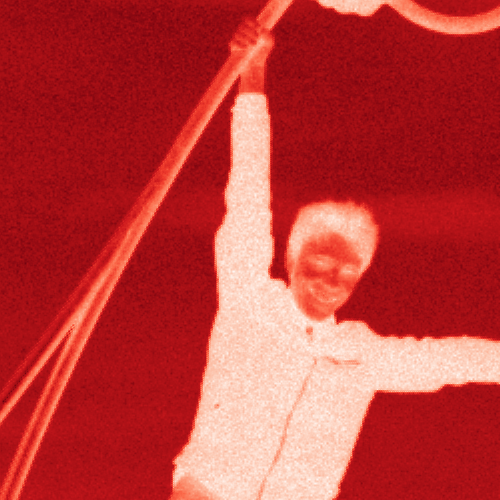
\includegraphics[width=0.9\textwidth]{src/assets/tests/red.png}
        \caption{Red channel}
        \label{fig:tests-red}
    \end{subfigure}
    \begin{subfigure}[b]{0.3\textwidth}
        \centering
        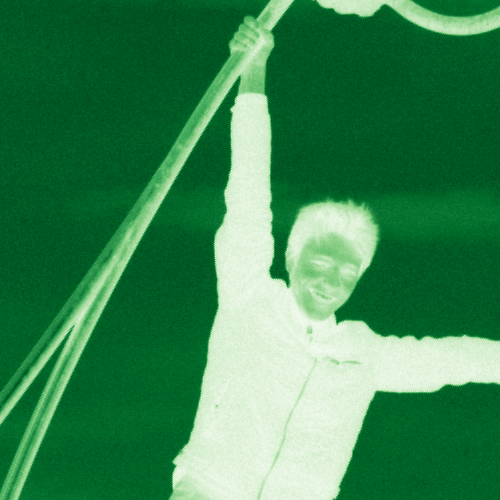
\includegraphics[width=0.9\textwidth]{src/assets/tests/green.png}
        \caption{Green channel}
        \label{fig:tests-green}
    \end{subfigure}
    \begin{subfigure}[b]{0.3\textwidth}
        \centering
        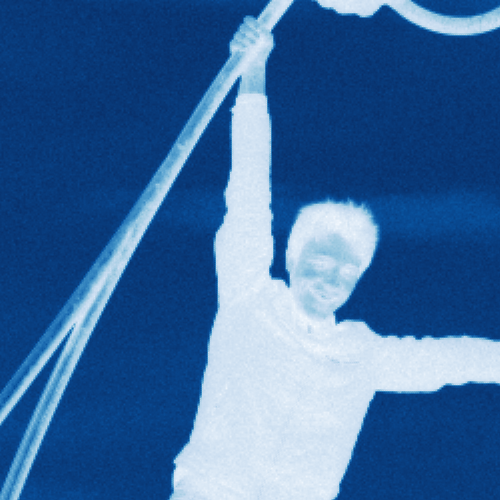
\includegraphics[width=0.9\textwidth]{src/assets/tests/blue.png}
        \caption{Blue channel}
        \label{fig:tests-blue}
    \end{subfigure}
    \caption{RGB Color space}
    \label{fig:tests-rgb}
\end{figure}

\begin{figure}[H]
    \centering
    \begin{subfigure}[b]{0.3\textwidth}
        \centering
        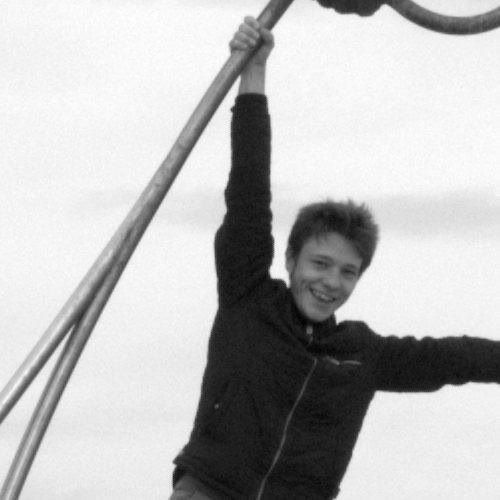
\includegraphics[width=0.9\textwidth]{src/assets/tests/Y.png}
        \caption{Y channel}
        \label{fig:tests-Y}
    \end{subfigure}
    \begin{subfigure}[b]{0.3\textwidth}
        \centering
        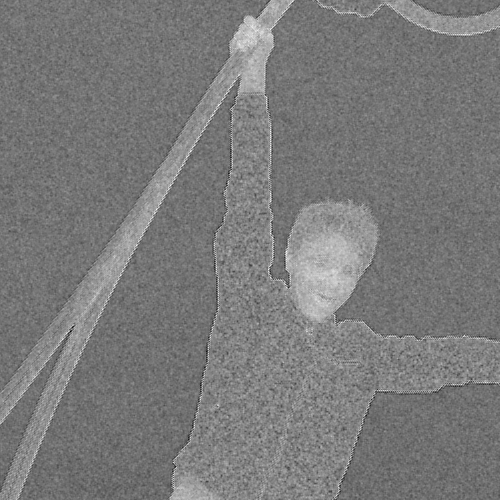
\includegraphics[width=0.9\textwidth]{src/assets/tests/Cr.png}
        \caption{Cr channel}
        \label{fig:tests-Cr}
    \end{subfigure}
    \begin{subfigure}[b]{0.3\textwidth}
        \centering
        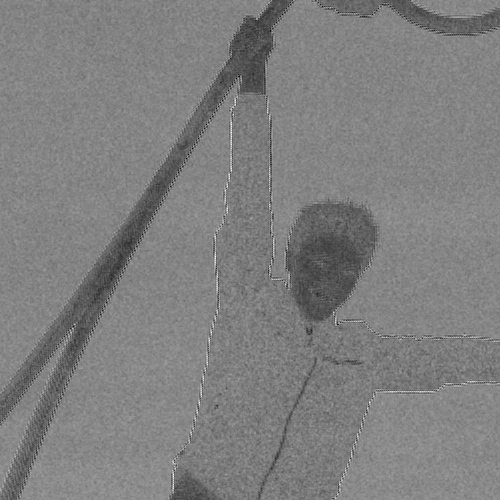
\includegraphics[width=0.9\textwidth]{src/assets/tests/Cb.png}
        \caption{Cb channel}
        \label{fig:tests-Cb}
    \end{subfigure}
    \caption{YCrCb color space}
    \label{fig:tests-yuv}
\end{figure}


\subsection{Downsampling chrominance channels}

\cFF{src/part-01/assets/step-2.py}{Downsampling}{downsampling}
We downsample the chrominance channels, by taking only one pixel every 2x2 pixels.
We can do this because the human eye is more sensitive to luminance than to chrominance.

\begin{figure}[H]
    \centering
    \begin{subfigure}[t]{0.4\textwidth}
        \centering
        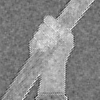
\includegraphics[width=\linewidth]{src/assets/tests/Cr_zoom.png}
        \caption{Cr original}
        \label{fig:tests-Cr-original}
    \end{subfigure}
    \hfill
    \begin{subfigure}[t]{0.4\textwidth}
        \centering
        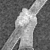
\includegraphics[width=\linewidth]{src/assets/tests/Cr_downsampled_zoom.png}
        \caption{Cr downsampled}
        \label{fig:tests-Cr-downsampled}
    \end{subfigure}

    \medskip

    \begin{subfigure}[t]{0.4\textwidth}
        \centering
        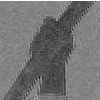
\includegraphics[width=\linewidth]{src/assets/tests/Cb_zoom.png}
        \caption{Cb original}
        \label{fig:tests-Cb-original}
    \end{subfigure}
    \hfill
    \begin{subfigure}[t]{0.4\textwidth}
        \centering
        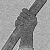
\includegraphics[width=\linewidth]{src/assets/tests/Cb_downsampled_zoom.png}
        \caption{Cb downsampled}
        \label{fig:tests-Cb-downsampled}
    \end{subfigure}


    \caption{YCrCb downsampled}
    \label{fig:tests-yuv-downsampled}
\end{figure}

\subsection{Compute DCT of blocks}

For each channel (Y, Cr, Cb) we slice the image into blocks of 8x8 pixels.
If the image size is not a multiple of 8, we have to add paddings to the image.
I choose a very simple solution by adding white borders (cf. Code \ref{code:pad}).
Then, we compute the DCT of each block.

\cFF{src/part-01/assets/pad.py}{Add padding}{pad}
\cFF{src/part-01/assets/step-3.py}{Compute DCT}{compute-dct}

To compute the dtc of the block, I tried to
reimplement it myself (Code \ref{code:dct}), but it is very very long
so I simply used the one from \iCode{cv2}.


\cFF{src/part-01/assets/dct.py}{DCT function}{dct}

\subsection{Quantization}

\cFF{src/part-01/assets/step-4.py}{Quantization}{quantization}
We quantize the DCT coefficients with a matrix of quantization.
I used a standard matrix of quantization.
I computed other matrices depending on the quality of compression (Code \ref{code:mat-comp}).

\cFF{src/part-01/assets/q.py}{Compression ratio}{mat-comp}

\begin{figure}[H]
    \centering
    \begin{subfigure}[t]{0.4\textwidth}
        \centering
        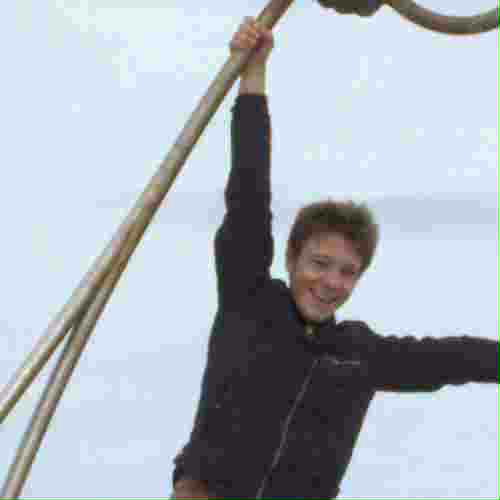
\includegraphics[width=\linewidth]{src/assets/tests/reconstructed_0.9.png}
        \caption{Compression ratio 90\%}
        \label{fig:tests-comp-0.1}
    \end{subfigure}
    \hfill
    \begin{subfigure}[t]{0.4\textwidth}
        \centering
        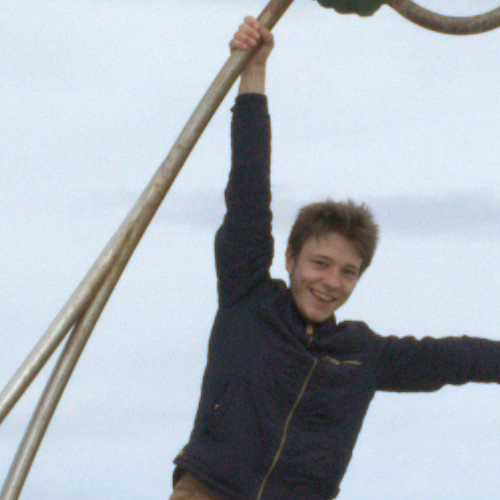
\includegraphics[width=\linewidth]{src/assets/tests/reconstructed_0.1.png}
        \caption{Compression ratio 10\%}
        \label{fig:tests-comp-0.9}
    \end{subfigure}


    \caption{Compression}
    \label{fig:tests-comp}
\end{figure}

